\documentclass[12pt,a4paper]{article}

\usepackage[
    a4paper,
    top=3cm,
    bottom=3cm,
    left=2.22cm,
    right=2.11cm,
    columnsep=1.27cm,
    footskip=1.2cm
]{geometry}
\usepackage[T1]{fontenc}
\usepackage[utf8]{inputenc}
\usepackage{amsmath}
\usepackage{amsfonts}
\usepackage{amssymb}
\usepackage{newtxtext,newtxmath}
\usepackage{helvet}
\usepackage{setspace}
\usepackage{microtype}
\usepackage[round,authoryear]{natbib}
\usepackage{graphicx}
\usepackage{textcomp}
\usepackage{caption}
\usepackage{subcaption}
\usepackage{titlesec}
\usepackage{dblfloatfix}
\usepackage{cuted}
\usepackage{placeins}
\usepackage[hidelinks,hypertexnames=false]{hyperref}
\usepackage{fancyhdr}
\usepackage{listings}
\usepackage{xcolor}
\usepackage{float}
\usepackage{array}
\usepackage{booktabs}
\usepackage{multirow}
\usepackage{url}
\usepackage{tikz}
\usetikzlibrary{arrows.meta,positioning,shapes.geometric}

\newcommand{\paperTitle}{Implementation and Evaluation of an Actual-Usage Pre-Eviction Filter for Kubernetes Descheduler}
\newcommand{\paperAuthors}{Matthew Hotmaraja Johan Turnip and Made Harta Dwijaksara}
\newcommand{\paperAffiliation}{Faculty of Computer Science, Universitas Indonesia}

\setlength{\parindent}{0.5in}
\setlength{\parskip}{0pt}
\setlength{\columnsep}{1.27cm}
\setlength{\headheight}{15pt}
\raggedbottom
\emergencystretch=2em

\titleformat{\section}
    {\normalfont\bfseries}
    {\thesection}
    {1em}
    {\MakeUppercase}
\titleformat{\subsection}
    {\normalfont\bfseries}
    {\thesubsection}
    {1em}
    {}
\titleformat{\subsubsection}
    {\normalfont\bfseries}
    {\thesubsubsection}
    {1em}
    {}
\titlespacing*{\section}{0pt}{1.2\baselineskip}{0.4\baselineskip}
\titlespacing*{\subsection}{0pt}{0.9\baselineskip}{0.25\baselineskip}
\titlespacing*{\subsubsection}{0pt}{0.7\baselineskip}{0.2\baselineskip}

\captionsetup{
    font=small,
    labelfont=bf,
    labelsep=period,
    justification=centering
}

\lstset{
    basicstyle=\scriptsize\ttfamily,
    breaklines=true,
    breakatwhitespace=true,
    columns=fullflexible,
    keepspaces=true,
    showstringspaces=false,
    frame=single,
    captionpos=b,
    numbers=left,
    numberstyle=\tiny,
    xleftmargin=1.0em,
    framexleftmargin=0.6em,
    breakindent=0pt,
    escapeinside={(*}{*)},
    postbreak=\mbox{\textcolor{gray}{$\hookrightarrow$}\space}
}

\let\cite\citep
\renewcommand{\refname}{References}

\fancypagestyle{uiarticle}{
    \fancyhf{}
    \fancyhead[R]{\thepage}
    \fancyfoot[R]{\fontsize{10}{12}\selectfont\sffamily\bfseries Universitas Indonesia}
    \renewcommand{\headrulewidth}{0pt}
    \renewcommand{\footrulewidth}{0pt}
}

\newcommand{\makeArticleFront}{%
    \newgeometry{top=3cm,bottom=3cm,left=2.38cm,right=3cm}
    \pagenumbering{arabic}
    \setcounter{page}{1}
    \pagestyle{uiarticle}
    \singlespacing
    \begin{center}
        {\bfseries \paperTitle\par}
        \vspace{0.6\baselineskip}
        {\paperAuthors\par}
        \vspace{0.25\baselineskip}
        {\paperAffiliation\par}
    \end{center}

    \vspace{0.8\baselineskip}
    \begin{center}
        \bfseries\MakeUppercase{Abstract}
    \end{center}
    \noindent
    Kubernetes Descheduler strategies select Pods using declared resources and
    placement state, but a selected Pod may be serving high live demand when
    eviction is attempted. This paper implements an Actual Usage Evictor as a
    global pre-eviction filter that compares live CPU and memory consumption
    with each Pod's effective resource requests. The filter blocks eviction
    when either request-relative usage ratio reaches a configurable threshold
    and fails closed when runtime metrics are unavailable or incomplete. We
    evaluate the implementation with two upstream strategies that pursue
    opposing placement objectives: \textit{HighNodeUtilization} for
    consolidation and \textit{LowNodeUtilization} for load redistribution.
    Four controlled systems, each represented by one independent run, are
    tested under sustained traffic to a single-replica, CPU-bound API. Without
    runtime filtering, evicting the busy API causes HTTP failure rates of
    \(16.67\%\) and \(17.24\%\), with observed failure spans of \(4.836\,s\)
    and \(4.873\,s\). With the filter enabled, both evaluated treatments retain
    the original API Pod and record no failed request.
    The placement cost depends on fallback availability:
    \textit{HighNodeUtilization} reduces the active-Node count by two instead
    of three, whereas \textit{LowNodeUtilization} substitutes an idle candidate,
    completes the same three evictions, and preserves the measured
    \(85.7\%\) memory-deviation reduction. These results show that a
    request-relative runtime guard can protect application availability while
    allowing the host strategy to continue whenever a compatible idle
    candidate exists in these tested layouts.

    \vspace{0.6\baselineskip}
    \noindent\textit{Keywords: Kubernetes, Descheduler, Pre-Eviction Filtering,
    Runtime Resource Usage, Service Availability}
}

\begin{document}

\makeArticleFront

\clearpage
\restoregeometry
\twocolumn
\singlespacing
\pagestyle{uiarticle}

\section{Introduction}
\label{sec:introduction}

Kubernetes places a Pod by filtering feasible Nodes and scoring the remaining
alternatives. CPU and memory requests determine placement feasibility, while
resource limits constrain runtime consumption after placement. Once bound, a
running Pod normally remains on its Node until it terminates or is recreated.
The Kubernetes Descheduler complements this behavior by evicting selected Pods
and allowing the kube-scheduler to place their replacements
\citep{k8s_descheduler_docs,larsson_klein_elmroth_2023}.

Placement information alone does not describe the operational cost of an
eviction. A Pod that is an attractive candidate under a consolidation or
load-balancing objective may be processing substantial live demand at the
moment the Descheduler acts. Eviction terminates that instance, after which a
replacement must be scheduled, started, marked Ready, and reattached to
traffic. For a single-replica service, this interval can directly become a
user-visible outage. In this paper, ``single-replica'' specifically means that
the \textit{workload-api} Deployment has one replica Pod behind its Service.

Runtime usage and scheduler feasibility answer different questions. Declared
requests determine where a replacement can fit, whereas current usage
indicates whether disrupting the selected instance is likely to remove active
service capacity. Replacing request-based strategy logic with instantaneous
usage would blur these concerns and make placement decisions sensitive to
short-lived measurements. A more composable approach is to retain the strategy
decision and add a runtime safety gate immediately before eviction.

This paper addresses the following research questions:

\begin{description}
    \item[\textbf{RQ1.}] Does the Actual Usage Evictor prevent
    eviction-induced application failure when a strategy selects a busy
    single-replica API Pod?
    \item[\textbf{RQ2.}] What placement cost does this protection impose under
    consolidation and load-redistribution objectives?
\end{description}

It makes three contributions:

\begin{itemize}
    \item an implementation of the Actual Usage Evictor as a global
    \textit{PreEvictionFilter}, independently composable with Descheduler
    strategies;
    \item a CPU-memory decision model with explicit handling for incomplete
    metrics and missing request baselines; and
    \item a controlled, CPU-path evaluation across the opposing objectives of
    \textit{HighNodeUtilization} and \textit{LowNodeUtilization}, separating
    application protection from strategy-specific placement cost.
\end{itemize}

The evaluation focuses on filter behavior rather than selecting an optimal
threshold. It compares controls using the Default Evictor with treatments that
add the Actual Usage Evictor while holding workload, layout, and host strategy
constant.

\section{Background and Related Work}
\label{sec:background}

\subsection{Kubernetes Resource Semantics}

A container may declare CPU and memory requests, limits, both, or neither.
Requests form the scheduler's placement baseline: a Pod is feasible on a Node
only when its effective requests fit the Node's remaining allocatable
resources. Limits instead define enforcement ceilings used by the kubelet and
container runtime \citep{k8s_resource_management}. A namespace
\textit{LimitRange} may insert defaults during admission, and those effective
values are visible in the stored Pod specification
\citep{k8s_limit_range}.

Requests and limits also contribute to Pod Quality of Service classification,
but QoS is not a direct proxy for current work. A \textit{Burstable} Pod can
legitimately consume far more CPU than its request when its limit permits it,
while a Pod with a large request can be idle
\citep{k8s_pod_qos}. Runtime protection therefore requires an observation of
current consumption as well as a baseline against which to interpret it.

Metrics Server exposes recent CPU and memory usage through the Kubernetes
Metrics API \citep{k8s_metrics_server}. CPU usage is represented in cores or
millicores and memory in bytes. These observations are point-in-time,
best-effort signals rather than reservations, so unavailable or incomplete
measurements require an explicit safety policy.

\subsection{Descheduling and Runtime Awareness}

The Descheduler runs after initial placement and proposes Pod evictions
according to a configured strategy. Before the eviction request reaches the
Kubernetes API, evictor plugins can enforce general eligibility and
pre-eviction checks. Multiple pre-eviction filters may be chained, so every
enabled filter must permit the candidate
\citep{k8s_descheduler_docs}. This extension point allows runtime protection
to remain independent of candidate ordering and the strategy's placement
objective.

Runtime telemetry has been used to revise Kubernetes placement at several
decision stages. The closest work combines load-aware scheduler scoring with a
custom Descheduler evictor that uses CPU, memory, network, and disk telemetry
to select the Pod with the greatest positive placement-score improvement
\citep{marchese2025enhancing}. An earlier network-aware scheduler and
Descheduler operator similarly uses measured latency and inter-service traffic
to evict a Pod when another Node offers a better score
\citep{marchese2022network}. Kinitos uses policy-specific scheduler and
Descheduler plugins to identify violated network dependencies and trigger
rescheduling, retaining the current placement when no feasible destination
exists \citep{tsokov2025kinitos}. Outside the Descheduler framework, Nautilus
uses runtime QoS and resource pressure to select and migrate a microservice
through a scale-out-before-delete workflow \citep{fu2022adaptive}. These
systems use telemetry for scoring, candidate selection, destination selection,
or managed migration. The Actual Usage Evictor operates at a narrower stage:
after a host strategy selects a candidate and immediately before eviction, its
global \textit{PreEvictionFilter} only permits or blocks that candidate. It
does not select, rank, place, or migrate Pods; it compares live CPU and memory
with effective requests and fails closed when metrics are unavailable or
incomplete.

The objective also differs from kubelet node-pressure eviction. Under resource
pressure, the kubelet ranks Pods to reclaim a scarce Node resource using Pod
Priority, whether usage exceeds requests, and usage relative to requests
\citep{k8s_node_pressure_eviction}. The Actual Usage Evictor is not a
reclamation mechanism for an unhealthy Node. It protects a busy candidate from
a voluntary, strategy-driven Descheduler eviction.

\subsection{Research Gap}

Prior work demonstrates that runtime telemetry can define or repair placement
through scoring, candidate selection, destination selection, and migration.
The architectural gap addressed here is a strategy-independent, global
pre-eviction veto that leaves candidate ordering and placement objectives to
the host Descheduler strategy. The Actual Usage Evictor occupies this narrower
boundary by checking request-relative live usage immediately before eviction
and defining fail-closed behavior when the required runtime evidence is
unavailable or incomplete.

\begin{figure*}[t]
    \centering
    \resizebox{\textwidth}{!}{%
        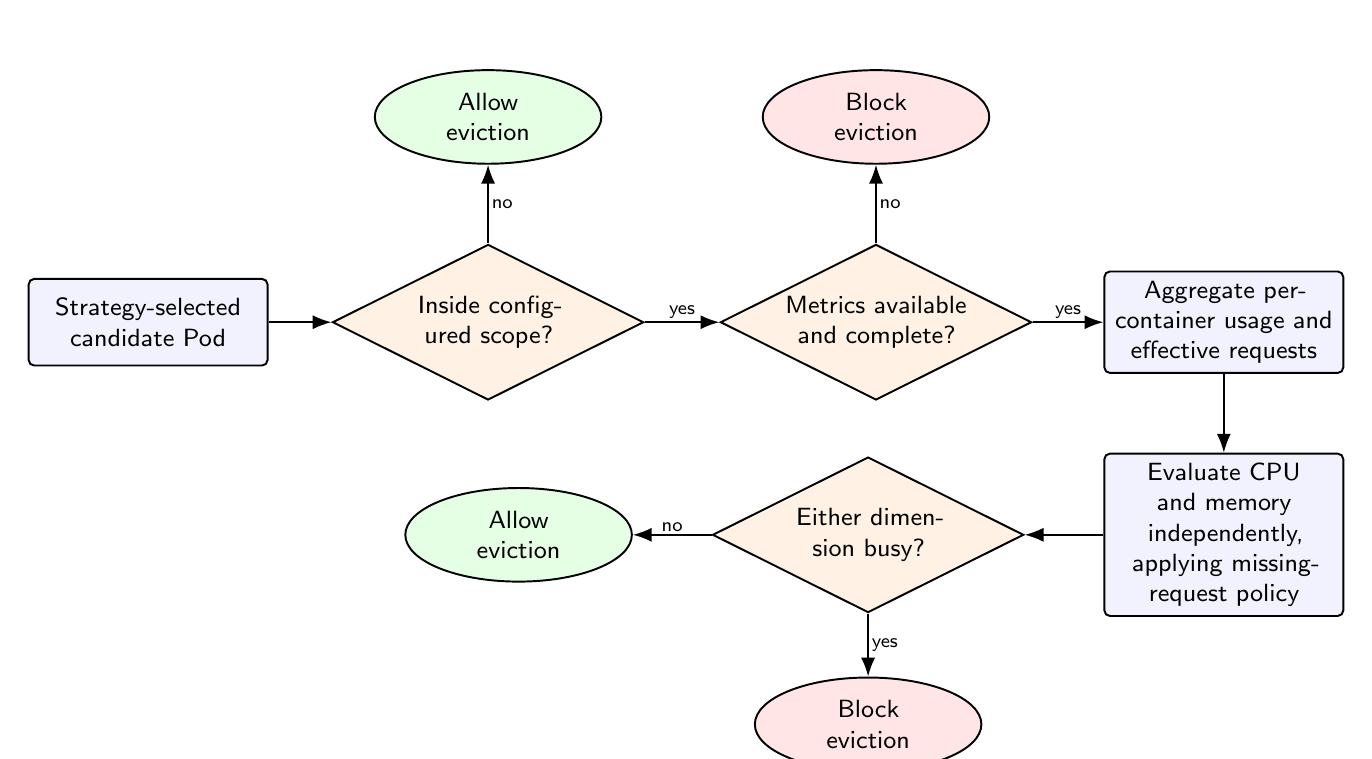
\begin{tikzpicture}[
    font=\sffamily\small,
    flow/.style={
        rectangle,
        rounded corners=2pt,
        draw=black,
        line width=0.7pt,
        align=center,
        minimum height=1.1cm,
        text width=2.8cm,
        fill=blue!5
    },
    decision/.style={
        diamond,
        aspect=2.0,
        draw=black,
        line width=0.7pt,
        align=center,
        inner sep=1.5pt,
        text width=2.3cm,
        fill=orange!10
    },
    terminal/.style={
        ellipse,
        draw=black,
        line width=0.7pt,
        align=center,
        minimum height=0.9cm,
        text width=1.8cm,
        fill=green!10
    },
    block/.style={
        ellipse,
        draw=black,
        line width=0.7pt,
        align=center,
        minimum height=0.9cm,
        text width=1.8cm,
        fill=red!10
    },
    arrow/.style={-{Latex[length=2.4mm]}, line width=0.7pt},
    label/.style={font=\sffamily\scriptsize, fill=white, inner sep=1pt}
]

\node[flow] (candidate) {Strategy-selected\\candidate Pod};
\node[decision, right=0.8cm of candidate] (scope) {Inside configured scope?};
\node[decision, right=0.95cm of scope] (metrics) {Metrics available and complete?};
\node[flow, right=0.9cm of metrics] (aggregate) {Aggregate per-container usage and effective requests};
\node[flow, below=1.0cm of aggregate] (evaluate) {Evaluate CPU and memory independently, applying missing-request policy};
\node[decision, left=1.0cm of evaluate] (busy) {Either dimension busy?};
\node[terminal, left=1.0cm of busy] (allow) {Allow eviction};
\node[block, below=0.8cm of busy] (deny) {Block eviction};
\node[terminal, above=1.0cm of scope] (outscope) {Allow eviction};
\node[block, above=1.0cm of metrics] (nometrics) {Block eviction};

\draw[arrow] (candidate) -- (scope);
\draw[arrow] (scope) -- node[label, above] {yes} (metrics);
\draw[arrow] (metrics) -- node[label, above] {yes} (aggregate);
\draw[arrow] (aggregate) -- (evaluate);
\draw[arrow] (evaluate) -- (busy);
\draw[arrow] (busy) -- node[label, above] {no} (allow);
\draw[arrow] (busy) -- node[label, right] {yes} (deny);
\draw[arrow] (scope) -- node[label, right] {no} (outscope);
\draw[arrow] (metrics) -- node[label, right] {no} (nometrics);

\end{tikzpicture}

    }
    \caption{Actual Usage Evictor pre-eviction decision flow. Request dimensions
    are evaluated independently, while unavailable or incomplete runtime
    metrics block the eviction.}
    \label{fig:actualusage_workflow}
\end{figure*}

\section{Actual Usage Evictor Implementation}
\label{sec:implementation}

\subsection{Plugin Position and Scope}

The Actual Usage Evictor implements the Descheduler \textit{EvictorPlugin}
interface. Its general \textit{Filter} method is a no-op that returns true;
runtime usage is evaluated only in \textit{PreEvictionFilter}. Candidate
selection therefore remains the responsibility of the active strategy. The
plugin observes the selected Pod immediately before eviction and either allows
the pipeline to continue or rejects that candidate.

\begin{table*}[t]
    \centering
    \caption{Actual Usage Evictor Parameters}
    \label{tab:actualusage_parameters}
    \small
    \renewcommand{\arraystretch}{1.2}
    \begin{tabular}{@{}p{3.9cm}p{1.5cm}p{1.6cm}p{7.9cm}@{}}
        \toprule
        \textbf{Parameter} & \textbf{Type} & \textbf{Default} & \textbf{Behavior} \\
        \midrule
        \textit{cpuUsageThreshold} & float & \(0.80\) &
        Blocks when actual CPU divided by effective requested CPU reaches the threshold. \\
        \textit{memoryUsageThreshold} & float & \(0.80\) &
        Blocks when actual memory divided by effective requested memory reaches the threshold. \\
        \textit{missingRequestPolicy} & string & Allow &
        Skips a missing request dimension under \textit{Allow}; rejects it under \textit{Block}. \\
        \textit{namespaces} & object & optional &
        Restricts evaluation with namespace include or exclude rules. \\
        \textit{labelSelector} & object & optional &
        Restricts evaluation using Kubernetes label matching. \\
        \bottomrule
    \end{tabular}
\end{table*}

Operators can restrict protection with namespace include or exclude rules and
a Kubernetes label selector. A Pod outside the configured scope passes without
a metrics query. When both controls are present, both must match for the
runtime check to run. This permits targeted protection of user-facing or
latency-sensitive workloads while leaving batch workloads unaffected.

Figure~\ref{fig:actualusage_workflow} shows the decision flow. For an in-scope
Pod, the plugin reads Pod metrics and matches each regular container in the
metric response with the Pod specification. Usage and effective requests are
aggregated only after every container has a complete CPU and memory
observation.

\subsection{Request-Relative Usage Model}

For Pod \(p\), let \(A_{p,c}\) and \(A_{p,m}\) denote aggregate actual CPU and
memory usage. Let \(R_{p,c}\) and \(R_{p,m}\) denote effective CPU and memory
requests aggregated across all regular containers. For a dimension in which
every container has a request, the ratios are

\[
\rho_{p,c}=\frac{A_{p,c}}{R_{p,c}},
\qquad
\rho_{p,m}=\frac{A_{p,m}}{R_{p,m}}.
\]

CPU is aggregated in millicores and memory in bytes. Effective requests are
read from the admitted Pod object, so defaults inserted by a
\textit{LimitRange} are included without a separate lookup.

Given CPU threshold \(\theta_c\) and memory threshold \(\theta_m\), the filter
blocks the eviction when either dimension reaches its threshold:

\[
\mathrm{Block}(p)
\iff
\rho_{p,c}\geq\theta_c
\;\lor\;
\rho_{p,m}\geq\theta_m.
\]

Consequently, both ratios must be below their thresholds for the candidate to
pass. The default \(\theta_c=\theta_m=0.80\) classifies activity relative to
the request baseline; it does not mean that the container is at \(80\%\) of
its runtime limit. A Pod with a \(50\,m\) CPU request and \(1000\,m\) limit can
produce a ratio far above one while legitimately bursting below its limit.
Limits are deliberately excluded because proximity to throttling or an
out-of-memory boundary is a different decision from activity relative to the
scheduler baseline.

The implementation applies this decision to both CPU and memory. The
experiments in Section~\ref{sec:evaluation}, however, generate foreground CPU
work and trigger the event from CPU samples; they validate the CPU decision
path only. The memory path was not evaluated independently.

\subsection{Missing Data and Safety Behavior}

Missing runtime evidence and missing request baselines have different
semantics. The plugin fails closed when the metrics client is unavailable,
Pod metrics cannot be read, or any regular container lacks a CPU or memory
observation. In these cases it cannot establish that eviction is safe.

If a container lacks an effective request for one resource, the entire
Pod-level dimension is marked missing rather than dividing by a partial
denominator. The dimension is then resolved using
\textit{missingRequestPolicy}. The default \textit{Allow} skips only that
dimension; the other dimension can still block through the OR condition.
\textit{Block} treats the missing dimension as busy. Thus, \textit{Allow} does
not claim that a request-less Pod is idle---it states that request-relative
busyness cannot be inferred for that dimension.

\subsection{Configuration}

Table~\ref{tab:actualusage_parameters} summarizes the public plugin arguments.
The complete decision procedure and an example policy are provided in
Appendices~\ref{appendix:actualusage_algorithm}
and~\ref{appendix:actualusage_config}.

\section{Evaluation Methodology}
\label{sec:evaluation}

\subsection{Experimental Setup and Procedure}

The testbed runs in an AWS Academy environment with one control-plane Node and
six \textit{t3.micro} worker Nodes. Each worker instance provides \(1\,GiB\) of
physical memory. After system and Kubernetes reservations, the recorded
allocatable capacity is approximately \(809\,Mi\) of memory and two CPU cores
per worker.

\begin{table*}[t]
    \centering
    \caption{Recorded Experimental Setup}
    \label{tab:experimental_setup}
    \small
    \renewcommand{\arraystretch}{1.15}
    \begin{tabular}{@{}>{\raggedright\arraybackslash}p{3.1cm}
        >{\raggedright\arraybackslash}p{12.4cm}@{}}
        \toprule
        \textbf{Item} & \textbf{Recorded configuration} \\
        \midrule
        Environment & AWS Academy; one control-plane Node and six
        \textit{t3.micro} workers, each with \(1\,GiB\) physical memory.
        Kubernetes allocatable capacity was two CPU cores and approximately
        \(809\,Mi\) memory per worker. \\
        Runtime components & Kubernetes cluster, Metrics Server through the
        Kubernetes Metrics API, a single-shot Descheduler Job, and
        \textit{k6} running outside the workload Pod through a NodePort. \\
        API workload & \textit{workload-api} Deployment with one replica Pod;
        \(50\,m\) CPU request, \(1000\,m\) CPU limit, \(700\,Mi\) memory limit;
        memory request \(240\,Mi\) (HNU) or \(200\,Mi\) (LNU). \\
        Traffic & Constant-arrival-rate at \(8\) requests/s to the API only.
        Each request executes a deterministic CPU-bound loop; the experiment
        does not generate memory load. \\
        Actual Usage policy & CPU and memory thresholds \(0.80\);
        \textit{missingRequestPolicy=Allow}; namespace
        \textit{actual-usage-exp}; label
        \textit{experiment=actual-usage-evictor}. \\
        Timing & \(30\,s\) stabilization; two consecutive CPU samples at least
        \(10\,s\) apart above threshold; \(30\,s\) post-event observation and
        analysis window \([0,30)\,s\). \\
        Experimental runs and reset & One independent run for each of H0, H1, L0,
        and L1. Each runner cleans previous state and rebuilds and validates
        the layout before its run. \\
        \bottomrule
    \end{tabular}
\end{table*}

Every run uses a \textit{workload-api} Deployment configured with one replica
Pod and exposed through a dedicated NodePort Service. A \textit{k6}
constant-arrival-rate workload sends approximately eight requests per second
only to this Service. Each request performs fixed CPU work. The API container
declares a \(50\,m\) CPU request, a \(1000\,m\) CPU limit, and a \(700\,Mi\)
memory limit; its memory request is \(240\,Mi\) in HNU and \(200\,Mi\) in LNU.
Other experiment Pods receive no foreground traffic.

The system stabilizes under load for \(30\,s\). The Kubernetes Metrics API is
then polled every \(10\,s\), and the Descheduler is triggered only after two
consecutive samples place the API CPU usage above the configured
\(0.80\) request-relative threshold. The decision-time CPU ratios are
approximately \(10.02\) in H1 and \(10.10\) in L1.

Immediately before the single-shot Descheduler Job starts, the experiment
records an event timestamp. Load generation and Pod lifecycle observation
continue for a \(30\,s\) post-event period. Application metrics are calculated
from requests completed in the event-aligned interval \([0,30)\,s\).

Table~\ref{tab:experimental_setup} summarizes values recorded by the runners,
policies, plans, and run artifacts. H0, H1, L0, and L1 are each one independent
run, not repeated trials. Before each run, the runner deletes prior experiment
state and recreates and validates the intended layout.

\subsection{Comparison Systems and Layouts}

The paired layouts are designed to compare filter behavior while holding the
workload, host strategy, traffic, and intended initial placement constant.
Each pair differs in whether the Actual Usage Evictor is registered after the
Default Evictor. Table~\ref{tab:comparison_systems} summarizes the four
configurations.

\begin{table*}[t]
    \centering
    \caption{H0, H1, L0, and L1 Configurations}
    \label{tab:comparison_systems}
    \small
    \renewcommand{\arraystretch}{1.2}
    \begin{tabular}{@{}l>{\raggedright\arraybackslash}p{2.4cm}
        >{\raggedright\arraybackslash}p{1.5cm}
        >{\raggedright\arraybackslash}p{4.3cm}
        >{\raggedright\arraybackslash}p{2.3cm}
        >{\raggedright\arraybackslash}p{3.5cm}@{}}
        \toprule
        \textbf{Run} & \textbf{Host / scheduler} &
        \textbf{Filter} & \textbf{Intended initial layout} &
        \textbf{Thresholds} & \textbf{Outcome} \\
        \midrule
        H0 & HNU / MostAllocated & Disabled &
        Three dense destinations; three one-Pod sources, with API alone on one source. &
        HNU CPU/memory \(40\%\) & Evictions, active Nodes, API identity,
        failures, failure span. \\
        H1 & HNU / MostAllocated & Enabled &
        Same intended layout as H0. &
        HNU \(40\%\); Actual Usage CPU/memory \(0.80\) & Same as H0 plus
        Actual Usage blocks. \\
        L0 & LNU / LeastAllocated & Disabled &
        Three underutilized destinations; three overutilized sources; API and
        idle fallback share one source. &
        LNU low \(20\%\), target \(50\%\) & Evictions, request deviation, API
        identity, failures, failure span. \\
        L1 & LNU / LeastAllocated & Enabled &
        Same intended layout as L0. &
        LNU \(20/50\%\); Actual Usage CPU/memory \(0.80\) & Same as L0 plus
        Actual Usage blocks. \\
        \bottomrule
    \end{tabular}
\end{table*}

\textit{HighNodeUtilization} (HNU) uses \textit{MostAllocated} scoring to pack
replacement Pods. In H0, the strategy can evict all three source Pods and
empty their Nodes. In H1, protecting the API prevents worker-6 from becoming
empty, but the two idle source Pods remain eligible.

\textit{LowNodeUtilization} (LNU) uses the default
\textit{LeastAllocated} scheduler. In both runs, the strategy attempts one
movement from each overutilized source. On worker-6 the busy API is considered
before an idle fallback. Therefore, L1 can reject the API and continue with
the fallback without reducing the successful eviction count.

\subsection{Metrics}

The Actual Usage Block Count \(B\) counts candidate rejections caused by a CPU
or memory ratio reaching its threshold. HTTP Failure Rate \(F\) is

\[
F=
\frac{N_{\mathrm{fail,post}}}
     {N_{\mathrm{completed,post}}},
\]

where a failure is a completed non-\(2xx\) response in the common post-event
window. Observed Failure Span \(S_f\) is the elapsed time from the first to the
last failed response:

\[
S_f=
\begin{cases}
t_{\mathrm{last\ fail}}-t_{\mathrm{first\ fail}},
    & N_{\mathrm{fail,post}}>0,\\
0, & N_{\mathrm{fail,post}}=0.
\end{cases}
\]

This quantity describes the temporal spread of observed failures, not the full
period of service unavailability or time to recovery. It is zero both when no
failure is observed and when only one failure occurs.

The evaluation also records successful eviction count, evicted Pod identity,
and whether the original API instance remains. For HNU, placement progress is
the reduction in active Nodes hosting non-DaemonSet application workloads.
For LNU, it is the reduction in the population deviation of normalized CPU
and memory requests across Nodes. Successful-request tail latency is treated
as secondary because individual runs contain transient bursts before and
after the event; failure rate and observed failure span are the primary
availability evidence.

\section{Results and Discussion}
\label{sec:results}

\begin{table*}[t]
    \centering
    \caption{Consolidated Actual Usage Evictor Results}
    \label{tab:consolidated_results}
    \small
    \renewcommand{\arraystretch}{1.18}
    \begin{tabular}{@{}lccccp{6.0cm}@{}}
        \toprule
        \textbf{Run} & \textbf{Evictions} & \textbf{Blocks} &
        \textbf{Failure rate} & \textbf{Failure span} &
        \textbf{Strategy-specific outcome} \\
        \midrule
        H0 & 3 & 0 & \(40/240=16.67\%\) & \(4.836\,s\) &
        Active Nodes \(6\to3\); busy API evicted. \\
        H1 & 2 & 1 & \(0/240=0\%\) & \(0\,s\) &
        Active Nodes \(6\to4\); original API retained. \\
        L0 & 3 & 0 & \(40/232=17.24\%\) & \(4.873\,s\) &
        Memory deviation reduced \(85.7\%\); busy API evicted. \\
        L1 & 3 & 1 & \(0/240=0\%\) & \(0\,s\) &
        Same \(85.7\%\) reduction via idle fallback; original API retained. \\
        \bottomrule
    \end{tabular}
\end{table*}

\subsection{HighNodeUtilization}

H0 evicts all three source Pods, including the busy API, and reduces the
active-Node count from six to three. H1 allows both idle source Pods but
observes an API CPU ratio of approximately \(10.02\), blocks that candidate,
and reduces the active-Node count from six to four. The filter therefore does
not disable consolidation; it trades one additional reclaimable Node for
preserving the active service instance.

H0 completes \(240\) responses in the common window and returns \(40\) HTTP
\(503\) responses, a \(16.67\%\) failure rate. Those failures have an observed
span of \(4.836\,s\). H1 completes \(240\) responses without failure.

\subsection{LowNodeUtilization}

L0 evicts the busy API and one idle Pod from each of the other sources. L1
observes an API CPU ratio of approximately \(10.10\), rejects that candidate,
then permits the idle fallback on the same Node. Both configurations complete
three successful evictions and produce the same final request distribution.

Memory request deviation falls from \(0.21639\) to \(0.03091\) in both runs,
a reduction of \(0.18548\), or \(85.7\%\). CPU deviation is unchanged because
the layout creates imbalance through memory requests while candidate CPU
requests are equal. L0 completes \(232\) responses and returns \(40\) HTTP
\(503\) responses, a \(17.24\%\) failure rate with an observed failure span of
\(4.873\,s\). L1 completes \(240\) responses with no failure.

\subsection{Cross-Strategy Interpretation}

The treatment changes the decision for the busy API without making idle Pods
ineligible. The placement cost is determined by what the host strategy can do
next. HNU has no substitute on the protected one-Pod source, so that Node
remains active and consolidation is partial. LNU has an idle candidate on the
same source; it substitutes that candidate and preserves the complete measured
balancing result. Runtime protection and placement progress are therefore not
inherently opposed. They conflict only when the host strategy lacks a
compatible idle alternative.

\subsection{Limitations}

The experiments use controlled six-Node layouts, synthetic CPU-bound demand,
a single API replica, one traffic pattern, one threshold value, and one
independent run per configuration. The paired layouts support a direct
behavioral comparison but do not represent every workload mix or failure
recovery mechanism. A replicated service might mask instance replacement,
while stateful, memory-bound, or long-running requests could exhibit a
different failure profile.

The \(0.80\) threshold is evaluated as a decision setting, not optimized.
Metrics API observations are sampled rather than continuous and can lag rapid
load changes. Finally, only two upstream strategies are evaluated. They cover
opposing consolidation and redistribution objectives, but broader strategy
and scheduler combinations are needed before generalizing the placement-cost
results to production clusters.

\clearpage

\section{Conclusion and Future Work}
\label{sec:conclusion}

This paper implemented an Actual Usage Evictor as a global pre-eviction safety
gate for Kubernetes Descheduler. The plugin preserves the candidate ordering
and placement objective of the active strategy, but checks live CPU and memory
usage immediately before eviction. The implementation supports CPU and memory
ratios, while the present CPU-bound experiments empirically validate only the
CPU decision path. Request-relative thresholds distinguish currently active
Pods from idle candidates, while conservative handling of unavailable or
incomplete metrics prevents eviction without adequate runtime evidence.

In the evaluated single-replica API scenarios, each represented by one
independent run, the filter blocked the busy API and allowed idle candidates
to remain eligible. Controls produced failure rates of \(16.67\%\) and
\(17.24\%\) and observed failure spans of approximately \(4.8\,s\); both
treatments recorded no failed response. HNU retained one additional active
Node because no fallback existed on the protected source. LNU substituted an
idle Pod, completed the same three evictions, and retained the full \(85.7\%\)
memory-deviation reduction. For these CPU-bound workloads and tested layouts,
runtime filtering protected the original API instance while preserving
strategy progress when a compatible alternative candidate was available.

Future work should evaluate threshold sensitivity across differently
calibrated requests, incorporate temporal smoothing or multiple consecutive
samples into the filter itself, and study the trade-off between responsiveness
and stale observations. Evaluation should also cover replicated, stateful, and
production-derived workloads; heterogeneous Nodes; longer requests; and
additional Descheduler strategies. Finally, exposing block reasons and recent
usage ratios as metrics would improve operator visibility and support
workload-specific threshold tuning.


\bibliographystyle{apalike}
\bibliography{config/references}

\clearpage
\onecolumn
\appendix

\section{Actual Usage Pre-Eviction Filter Algorithm}
\label{appendix:actualusage_algorithm}
\lstinputlisting[
    caption={Unified Actual Usage Evictor decision workflow.},
    label={lst:actualusage_algorithm}
]{assets/codes/pseudos/actualusage/unifiedalgo.psu}

\section{Actual Usage Evictor Configuration}
\label{appendix:actualusage_config}
\lstinputlisting[
    caption={Example Descheduler configuration with the Actual Usage Evictor.},
    label={lst:actualusage_config}
]{assets/codes/pseudos/actualusage/config.psu}

\end{document}
